% Offizielle Beispieldatei für beamer-Vorlage aus tubslatex Version 0.3beta2
\documentclass{beamer}

\usepackage[english]{babel}
\usepackage[utf8]{inputenc}

\usetheme[%
  %nexus,%        Nexus Fonts benutzen
  %lnum,%         Versalziffern verwenden
  %cmyk,%<rgbprint>,          Auswahl des Farbmodells
  orange,%<orange/green/violet> Auswahl des Sekundärfarbklangs
  light,%<light,medium>        Auswahl der Helligkeit
  colorhead,%    Farbig hinterlegte Kopfleiste
  colorfoot,%    Farbig hinterlegt Fußleiste auf Titelseite
  colorblocks,%   Blöcke Farbig hinterlegen
  %nopagenum,%    Keine Seitennumer in Fußzeile
  %totalpages,%    Angabe der Gesamtseitenzahl in Fußzeile
  nodate,%       Kein Datum in Fußleiste
  %tocinheader,%   Inhaltsverzeichnis in Kopfleiste
  %tinytocinheader,% kleines Kopfleisten-Inhaltsverzeichnis
  %widetoc,%      breites Kopfleisten-Inhaltsverzeichnis
  %narrowtoc,%    schmales Kopfleisten-Inhaltsverzeichnis
  %nosubsectionsinheader,%  Keine subsections im Kopfleisten-Inhaltsverzeichnis
  nologoinfoot,% Kein Logo im Fußbereich darstellen
  ]{tubs}
\usepackage{tikz}
\usetikzlibrary{arrows.meta}

% BibLatex configuration
\usepackage{csquotes}
\usepackage[backend=biber,style=authoryear,giveninits=true,url=false,doi=false,isbn=false]{biblatex}
\addbibresource{bibliography.bib}
\setbeamertemplate{bibliography item}[text]

\setbeamertemplate{theorems}[numbered]
\setbeameroption{show notes}

% Titelseite
\title{Reducing density matrices: a geometric view}
\subtitle{\hfill Joint work with V. Bach}
\author{R. Rauch}
\date{Singapore, September 13, 2019}
\titlegraphic[scaled]{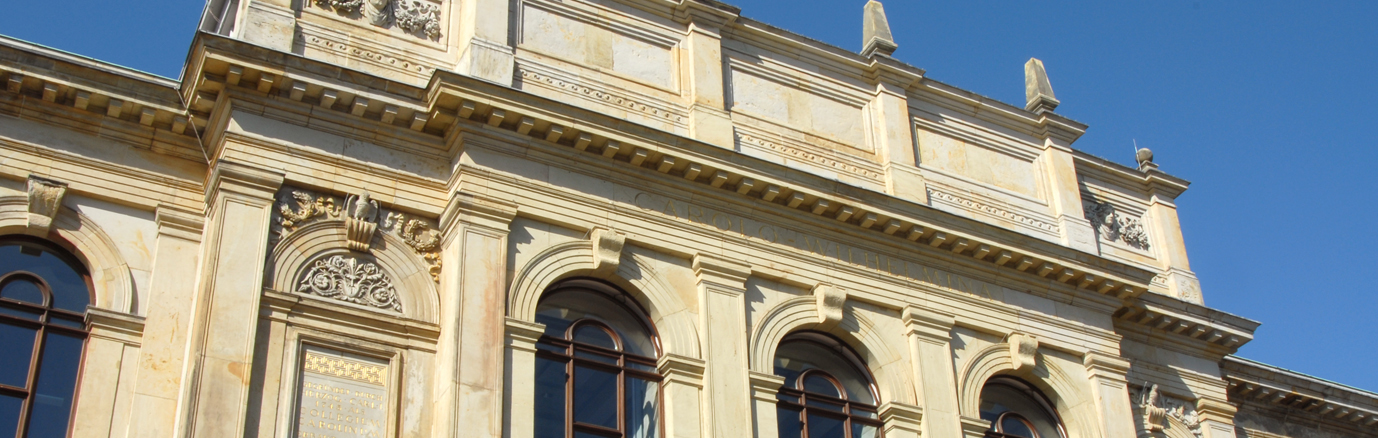
\includegraphics{titlepicture.jpg}}

\DeclareMathOperator{\tr}{tr}
\DeclareMathOperator{\pos}{pos}
\DeclareMathOperator{\spn}{span}
\DeclareMathOperator{\im}{im}
\newcommand{\IN}{\ensuremath{\mathbb{N}}}
\newcommand{\IZ}{\ensuremath{\mathbb{Z}}}
\newcommand{\IR}{\ensuremath{\mathbb{R}}}
\newcommand{\IC}{\ensuremath{\mathbb{C}}}
\newcommand{\IK}{\ensuremath{\mathbb{K}}}
\newcommand{\normord}[1]{:\mathrel{#1}:}
\newcommand{\card}[1]{{\ensuremath{\left|#1\right|}}}
\newcommand{\imag}{\mathrm{i}}
\newcommand{\CAR}[1]{{\ensuremath{\IC[c,c^*]}}}
\newcommand{\CARabs}[1]{{\ensuremath{\mathfrak{A}(#1)}}}
\newcommand{\one}{\mathbb{1}}
\newcommand{\N}{\mathbf{n}}
\newcommand{\C}{\mathbf{c}}
\newcommand{\Cd}{\C^*}
\newcommand{\PowerSet}[1]{\mathfrak{P}\left(#1\right)}
\newcommand{\HS}{{\mathcal{L}^2(\FockSpace)}}
\newcommand{\HSbasis}{\mathfrak{B}}
\newcommand{\HilbertSpace}{\ensuremath{\mathfrak{h}}}
\newcommand{\FockSpace}{\mathcal{F}}
\newcommand{\Vacuum}{\Omega_\FockSpace}
\newcommand{\sign}[2]{\begin{bmatrix}\begin{matrix}#1\end{matrix}\\\begin{matrix}#2\end{matrix}\end{bmatrix}}
\newcommand{\Hamiltonian}{\mathbb{H}}
\newcommand{\StateSpace}{\mathcal{S}}
\newcommand{\DensityMatrices}{\mathcal{DM}}

% space of k-body operators
\newcommand{\kbOp}[1][k]{{\ensuremath{\mathcal{O}_{#1}(\mathcal{F})}}}
\newcommand{\PkbOp}[1][k]{{\ensuremath{\pi_{#1}}}}
\newcommand{\kbOpBasis}[1][k]{\mathfrak{B}_{#1}}

% space of k-body observables
\newcommand{\kbOb}[1][k]{{\ensuremath{\mathcal{O}_{#1}^\mathbb{R}(\mathcal{F})}}}
\newcommand{\PkbOb}[1][k]{{\ensuremath{\pi_{#1}^\mathbb{R}}}}
\newcommand{\kbObBasis}[1][k]{\mathfrak{B}_{#1}}

\begin{document}

\begin{frame}[plain]
\titlepage
\end{frame}

\section{Motivation: The Representability Problem}
\subsection{Quantum Systems in Theoretical Chemistry}
\frame{\sectionpage}

\begin{frame}{Quantum Systems in Theoretical Chemistry}
    \begin{itemize}
        \item<1-> \textbf{Quantum chemistry}: \emph{molecules} as non-relativistic,
        many-fermion quantum systems (\emph{Born-Oppenheimer approximation})
        \begin{itemize}
            \item<2-> \textbf{Hilbert space:} Fermion Fock space
            \begin{equation}
                \mathcal{F}=\bigoplus_{N\ge 0}\bigwedge^N\HilbertSpace\qquad
                \begin{gathered}
                    \text{with }\HilbertSpace=\text{ $1$-particle Hilbert space},\\
                    \text{e.g. }\HilbertSpace=L^2(\IR^3)\otimes\IC^2
                \end{gathered}
            \end{equation}
            \item<3-> \textbf{Hamiltonian:} a \emph{2-body operator} $\Hamiltonian=\Hamiltonian^*=\bigoplus_{N\ge 0}\Hamiltonian_N$, e.g.
            \begin{equation}
                \Hamiltonian_N=
                \underbrace{\sum_{i=1}^N\left(-\Delta_i-\sum_{j=1}^K\frac{Z_j}{|x_i-R_j|}\right)}_{\text{1-particle ``free part''}}
                +\underbrace{\sum_{1\le i<j\le N}\frac{1}{|x_i-x_j|}}_{\text{2-particle ``interaction part''}}.
            \end{equation}
        \end{itemize}
    \end{itemize}
\end{frame}

\subsection{Reducing States: The Representability Problem}
\begin{frame}{Computing the Ground State Energy}
    \begin{block}{}<1->
        \textbf{Key Problem}: Compute the ground state energy
        \begin{equation}
            \label{GSE}
            E_0=\inf_{\rho\in\DensityMatrices}\tr\{\rho\Hamiltonian\},
            \quad\DensityMatrices\doteq\{\text{density matrices on }\FockSpace\}.
        \end{equation}
    \end{block}
    \begin{itemize}
        \item<2-> \textbf{Observe}: For $2$-body Hamiltonians $\Hamiltonian$ the variation over
        $\DensityMatrices$ is very inefficient
        \begin{itemize}
            \item<3-> general density matrix $\rho$ contains ``too much'' information
            \item<3-> only need expectation values of $2$-body operators
        \end{itemize}
        \item<4-> \textbf{More generally:} practically all physical relevant information can be obtained by
        2-body expectation values.
    \end{itemize}
\end{frame}

\begin{frame}{Reducing Density Matrices}
    \begin{block}{}<1->
        \textbf{Idea}: Replace density matrix $\rho\in\mathcal{B}(\FockSpace)'$ by its
        \emph{$2$-body reduction}
        \begin{equation}
            R_2(\rho)\doteq\rho|_{\kbOp[2]}\in\kbOp[2]'.
        \end{equation}
    \end{block}
    \begin{itemize}
        \item<2-> \textbf{Advantage:} If $\Hamiltonian\in\kbOp[2]$ then
        \begin{equation}
            E_0=\inf_{\rho\in\DensityMatrices}\rho(\Hamiltonian)=
            \inf_{r\in R_2(\DensityMatrices)}r(\Hamiltonian).
        \end{equation}
        %and $R_2(\DensityMatrices)$ is \emph{a lot} smaller than $\DensityMatrices$.\\[1em]
        \item<3-> \textbf{Drawback:} We need an efficient way of varying over $R_2(\DensityMatrices)$.
    \end{itemize}
\end{frame}

\begin{frame}{The Representability Problem}
    \begin{block}{Representability Problem (for $R_2(\DensityMatrices)$)}
        Find a \emph{computationally efficient} characterization of
        $R_2(\DensityMatrices)$:
        \begin{center}
            \textit{Given $r\in\kbOp[2]'$, is there $\rho\in\DensityMatrices$ with $r=R_2(\rho)$?}
        \end{center}
    \end{block}
    \begin{itemize}
        \item<2-> \textbf{Generalization:} $\DensityMatrices\rightsquigarrow\mathcal{S}\subseteq\mathcal{B}(\FockSpace)'$ and  $k=2\rightsquigarrow k\in\IN_0$: \emph{representability problem for $R_k(\mathcal{S})$}.
        \item<3-> \textbf{Representability conditions} (i.e. necessary conditions for representability) yield lower bounds on $E_0$.
    \end{itemize}
\end{frame}

\begin{frame}{Geometric Interpretation}
    \begin{block}{}
        \textbf{Note:} If $\dim\HilbertSpace<\infty$, then $R_k:\mathcal{B}(\FockSpace)'\to\kbOp'$ can be interpreted as the
        \emph{orthogonal projection}
        \begin{equation}
            \pi_k:\HS\to\kbOp\subseteq\HS.
        \end{equation}
    \end{block}
    \onslide<2->{
        \begin{center}
        \begin{tikzpicture}[scale=.6]
            % Convex set of density matrices
            \filldraw[fill=gray!20,very thick] (0,0) -- (2,0.5) -- (3,2.5) .. controls (3.2,4.5) .. (1,5)
            -- (-1,4) -- (-1.75,2) -- cycle;
            \draw (.8,2.5) node {$\DensityMatrices$};

            % Subspace of $k$-body operators
            \draw (8,-0.5) node[below] {$\kbOp$} -- (8,5.5);

            % Set or representable density matrices
            \draw[very thick,color=red] (8,0) -- node[left=5pt]{$\PkbOp(\DensityMatrices)$} (8,5);

            \draw[dashed] (1,5) -- (8,5);
            \draw[dashed] (0,0) -- (8,0);
        \end{tikzpicture}
        \end{center}
    }
\end{frame}

\begin{frame}{Some History of Representability Methods}
    \begin{itemize}
        \item \textbf{1940:} Idea to replace $\DensityMatrices$ by $R_2(\DensityMatrices$) (Husimi)
        \item \textbf{1950/60s:} First systematic analysis (Coleman, Coulson, Garrod, Percus, Löwdin, Yang)
        \begin{itemize}
            \item $GPQ$-conditions lead to inaccurate lower bounds
            \item solved Representability Problem for $R_1(\mathcal{SD}_N)$
        \end{itemize}
        \item \textbf{1978:} $T_1$- and $T_2$-conditions (Erdahl)
        \item \textbf{2005:} Representability of $R_1(\mathcal{P}_N)$ solved  (Klyachko)
        \item \textbf{2006:} Highly accurate lower bounds exploiting Erdahls $T_1$- and $T_2$-conditions (Cancés, Lewin, Stoltz)
        \item \textbf{2012:} Derivation of HF error estimates from $G$- and $P$-condition (Bach, Bretaux, Knörr, Menge)
    \end{itemize}
\end{frame}

\section{Orthogonalization of $k$-body Operators}\frame{\sectionpage}
\subsection{Goal}
\begin{frame}{Goal of Present Work}

\begin{itemize}
    \item \textbf{Wanted}: more explicit formula for $\pi_k$, e.g., by diagonalization:
    \begin{block}{Goal}<2->
        Construct an explicit orthonormal basis of $\kbOp$.
    \end{block}
    \item<3-> \textbf{Approach:}
    \begin{enumerate}
        \item Apply Gram-Schmidt orthogonalization in low dimensions
        \item Find and prove a general conjecture
    \end{enumerate}
\end{itemize}
\end{frame}

\subsection{Results}
\begin{frame}{Main Result}
    \begin{theorem}[\cite{Bach2018}]
        Let $\dim\HilbertSpace\doteq n<\infty$ and $\varphi_1,\ldots,\varphi_n$ an ONB of $\HilbertSpace$.
        Then an orthogonal basis of $\HS$ is given by
        \begin{equation}
            \HSbasis\doteq\left\{
            \left.\left(\prod_{k\in K}\left[c_k,c_k^*\right]\right)c_I^*c_J\;\right|
            \begin{gathered}
                I,J,K\subseteq\{1,\ldots,n\}\\\text{ mutually disjoint}
            \end{gathered}
            \right\},
        \end{equation}
        where for $I=\{i_1<\cdots<i_l\}\subseteq\{1,\ldots,n\}$ we define
        \begin{align}
            c_I^*&\doteq c^*(\varphi_{i_1})\cdots c^*(\varphi_{i_l}),&
            c_I&\doteq\left(c_I^*\right)^*=c(\varphi_{i_l})\cdots c(\varphi_{i_1}).
        \end{align}
    \end{theorem}
    \begin{theorem}<2->[\cite{Bach2018}]
        An orthogonal basis of $\kbOp$ is given by $\HSbasis\cap\kbOp$.
    \end{theorem}
\end{frame}

\begin{frame}{Main Result: Geometric Interpretation}
    \begin{itemize}
        \item \textbf{To Summarize:} We have constructed an ONB $\mathfrak{B}$ of
        $\HS$ adapted to the study of representability and related questions.
    \end{itemize}
    \begin{figure}
    \begin{tikzpicture}[scale=.6]
        % Convex set of density matrices
        \filldraw[fill=gray!20,very thick] (0,0) -- (2,0.5) -- (3,2.5) .. controls (3.2,4.5) .. (1,5)
        -- (-1,4) -- (-1.75,2) -- cycle;
        \draw (.8,2.5) node {$\DensityMatrices$};

        % Subspace of $k$-body operators
        \draw (8,-0.5) node[below] {$\kbOp$} -- (8,5.5);

        \draw[dashed,very thin] (1,5) -- (8,5);
        \draw[dashed] (0,0) -- (8,0);

        % visualize basis
        \draw[Stealth-Stealth, color=red, very thick] (8,2) -- node[left, near end]{$\HSbasis$} (8,0) -- (6,0);
    \end{tikzpicture}
\end{figure}
\end{frame}

\subsection{Current Research}
\begin{frame}{Current Research}
    \begin{enumerate}
        \item Characterize $\pi_k(\DensityMatrices)\subseteq\kbOp$ using the ONB $\HSbasis\cap\kbOp$
        \item Identify classical representability conditions as boundary conditions
        \item Obtain new representability conditions
        \item Study action of Bogoliubov transformations on representability conditions
    \end{enumerate}
\end{frame}

\begin{frame}{Possible Application}
    \begin{itemize}
        \item Consider a 2-body Hamiltonian $\Hamiltonian$, fix an ONB
        $\varphi_1,\dots,\varphi_n$ of $\HilbertSpace$ and write
        \begin{equation}
            \Hamiltonian=\sum_{i,j}t_{ij}c_i^*c_j+\frac{1}{2}\sum_{i,j,k,l}V_{ij;kl}c_i^*c_j^*c_lc_k,
        \end{equation}
        \item Let $\mathfrak{B}$ be the associated ONB of $\HS$ as given by Theorem 1
        \item For $\mathfrak{A}\subseteq\mathfrak{B}$ define
        $P_{\mathfrak{A}}\doteq\sum_{\theta\in\mathfrak{A}}\left|\theta\rangle\langle\theta\right|\le
        1_\HS$.
        \item Then, under suitable positivity requirements on $V$,
        \begin{equation}
            \Hamiltonian\ge\sum_{i,j}t_{ij}c_i^*c_j+
            \frac{1}{2}\sum_{i,j,k,l}V_{ij;kl}c_i^*c_j^*\textcolor{red}{P_\mathfrak{A}}c_lc_k
            \doteq\Hamiltonian_\mathfrak{A}.
        \end{equation}
        \item \textbf{Idea:} by a suitable choice
        of the orbital basis $\varphi_1,\ldots,\varphi_n$ and $\mathfrak{A}\subseteq\mathfrak{B}$
        one obtains nontrivial lower bound $E_0(\Hamiltonian_\mathfrak{A})$ of $E_0(\Hamiltonian)$.
    \end{itemize}
\end{frame}

\section{Appendix}
\frame{\sectionpage}

\begin{frame}{$k$-Body Operators}
\begin{definition}
    A \emph{$k$-body operator} on $\FockSpace$ is a $\IC$-linear
    combination of elements of the form
    \begin{equation}
        c^\sharp(f_1)\cdots c^\sharp(f_{2l})\qquad f_1,\ldots,f_{2\ell}\in\HilbertSpace
        \text{ and }0\le \ell\le k,
    \end{equation}
    with $c^*(f),c(f)\in\mathcal{B}(\FockSpace)$ the \emph{creation-} and \emph{annihilation operators} on $\FockSpace$.
\end{definition}
\end{frame}

\begin{frame}{Representability of $R_2(\DensityMatrices_N)$}
    \begin{exampleblock}{}
        Let $\rho\in\DensityMatrices_N\doteq\{\rho\in\DensityMatrices\mid\hat{\IN}\rho=N\rho\}$. Then $R_2(\rho)\in\kbOp[2]'$
        is characterized by
        \begin{align}
            \gamma_\rho&\in\mathcal{B}(\HilbertSpace),\tag{1-RDM}\\
            \Gamma_\rho&\in\mathcal{B}(\HilbertSpace\wedge\HilbertSpace).\tag{2-RDM}
        \end{align}
    \end{exampleblock}
    \begin{itemize}
        \item \textbf{$N$-Representability Problem}: Given $\gamma\in\mathcal{B}(\HilbertSpace)$
        and $\Gamma\in\mathcal{B}(\HilbertSpace\wedge\HilbertSpace)$,  is there $\rho\in\DensityMatrices$ with $\hat{\IN}\rho=N\rho$ such that
            \begin{align}
                \gamma&=\gamma_\rho&\Gamma&=\Gamma_\rho
            \end{align}
        \item Examples of \textbf{$N$-Representability conditions}:
        \begin{equation}
            \begin{aligned}
                0&\le\gamma_\rho\le 1,&
                \tr\{\gamma_\rho\}&=N,&
                \Gamma_\rho&\ge 0.
            \end{aligned}
        \end{equation}
    \end{itemize}
\end{frame}

\section*{References}
\begin{frame}{References}
    \nocite{*}
    \printbibliography
\end{frame}

\end{document}
